\documentclass[12pt, titlepage]{article}

%% Comments

\usepackage{color}

\newif\ifcomments\commentstrue

\ifcomments
\newcommand{\authornote}[3]{\textcolor{#1}{[#3 ---#2]}}
\newcommand{\todo}[1]{\textcolor{red}{[TODO: #1]}}
\else
\newcommand{\authornote}[3]{}
\newcommand{\todo}[1]{}
\fi

\newcommand{\wss}[1]{\authornote{blue}{SS}{#1}} 
\newcommand{\plt}[1]{\authornote{magenta}{TPLT}{#1}} %For explanation of the template
\newcommand{\an}[1]{\authornote{cyan}{Author}{#1}}

%% Common Parts
\usepackage{booktabs}
\usepackage{tabularx}
\usepackage{hyperref}
\usepackage[round]{natbib}
\usepackage{amsmath, mathtools}
\usepackage{amsfonts}
\usepackage{amssymb}
\usepackage{graphicx}
\usepackage{colortbl}
\usepackage{xr}
\usepackage{longtable}
\usepackage{xfrac}
\usepackage{float}
\usepackage{siunitx}
\usepackage{caption}
\usepackage{pdflscape}
\usepackage{afterpage}
\usepackage{tikz}
\usetikzlibrary{mindmap}
\usepackage{multirow}
\usepackage{fullpage}
%\usepackage{refcheck}

\newcommand{\famname}{MIA}
\newcommand{\progname}{MISEG}

% For easy change of table widths
\newcommand{\colZwidth}{1.0\textwidth}
\newcommand{\colAwidth}{0.13\textwidth}
\newcommand{\colBwidth}{0.82\textwidth}
\newcommand{\colCwidth}{0.1\textwidth}
\newcommand{\colDwidth}{0.05\textwidth}
\newcommand{\colEwidth}{0.8\textwidth}
\newcommand{\colFwidth}{0.17\textwidth}
\newcommand{\colGwidth}{0.5\textwidth}
\newcommand{\colHwidth}{0.28\textwidth}

% Used so that cross-references have a meaningful prefix
\newcounter{defnum} %Definition Number
\newcommand{\dthedefnum}{GD\thedefnum}
\newcommand{\dref}[1]{GD\ref{#1}}
\newcounter{datadefnum} %Datadefinition Number
\newcommand{\ddthedatadefnum}{DD\thedatadefnum}
\newcommand{\ddref}[1]{DD\ref{#1}}
\newcounter{theorynum} %Theory Number
\newcommand{\tthetheorynum}{T\thetheorynum}
\newcommand{\tref}[1]{T\ref{#1}}
\newcounter{tablenum} %Table Number
\newcommand{\tbthetablenum}{T\thetablenum}
\newcommand{\tbref}[1]{TB\ref{#1}}
\newcounter{assumpnum} %Assumption Number
\newcommand{\atheassumpnum}{P\theassumpnum}
\newcommand{\aref}[1]{A\ref{#1}}
\newcounter{goalnum} %Goal Number
\newcommand{\gthegoalnum}{P\thegoalnum}
\newcommand{\gsref}[1]{GS\ref{#1}}
\newcounter{instnum} %Instance Number
\newcommand{\itheinstnum}{IM\theinstnum}
\newcommand{\iref}[1]{IM\ref{#1}}
\newcounter{reqnum} %Requirement Number
\newcommand{\rthereqnum}{P\thereqnum}
\newcommand{\rref}[1]{R\ref{#1}}
\newcounter{lcnum} %Likely change number
\newcommand{\lthelcnum}{LC\thelcnum}
\newcommand{\lcref}[1]{LC\ref{#1}}

\hypersetup{
    bookmarks=true,         % show bookmarks bar?
    colorlinks=true,       % false: boxed links; true: colored links
    linkcolor=red,          % color of internal links (change box color with linkbordercolor)
    citecolor=green,        % color of links to bibliography
    filecolor=magenta,      % color of file links
    urlcolor=cyan           % color of external links
}


\begin{document}

\title{Module Guide for \progname{}} 
\author{Ao Dong}
\date{\today}

\maketitle

\pagenumbering{roman}

\section{Revision History}

\begin{tabularx}{\textwidth}{p{3cm}p{2cm}X}
\toprule {\bf Date} & {\bf Version} & {\bf Notes}\\
\midrule
Nov 25 & 1.0 & Initial draft\\
Dec 11 & 1.1 & Modification according to feedback\\
\bottomrule
\end{tabularx}

\newpage

\section{Reference Material}

This section records information for easy reference.

\subsection{Abbreviations and Acronyms}

\renewcommand{\arraystretch}{1.2}
\begin{tabular}{l l} 
  \toprule		
  \textbf{symbol} & \textbf{description}\\
  \midrule 
  1D & one-dimensional\\
  3D & three-dimensional\\
  AC & Anticipated Change\\
  DAG & Directed Acyclic Graph \\
  dcm4che & A DICOM Toolkit and Library\\
  M & Module \\
  MG & Module Guide \\
  $\mathbb{N}$ & Natural Number\\
  OS & Operating System \\
  R & Requirement\\
  SC & Scientific Computing \\
  SRS & Software Requirements Specification\\
  \progname & Explanation of program name\\
  UC & Unlikely Change \\
  \bottomrule
\end{tabular}\\

\newpage

\tableofcontents

\listoftables

\listoffigures

\newpage

\pagenumbering{arabic}

\section{Introduction}

Decomposing a system into modules is a commonly accepted approach to developing
software.  A module is a work assignment for a programmer or programming
team~\citep{ParnasEtAl1984}.  We advocate a decomposition
based on the principle of information hiding~\citep{Parnas1972}.  This
principle supports design for change, because the ``secrets'' that each module
hides represent likely future changes.  Design for change is valuable in SC,
where modifications are frequent, especially during initial development as the
solution space is explored.  

Our design follows the rules layed out by \citet{ParnasEtAl1984}, as follows:
\begin{itemize}
\item System details that are likely to change independently should be the
  secrets of separate modules.
\item Each data structure is implemented in only one module.
\item Any other program that requires information stored in a module's data
structures must obtain it by calling access programs belonging to that
module.\end{itemize}

After completing the first stage of the design, the Software Requirements
Specification (SRS), the Module Guide (MG) is developed~\citep{ParnasEtAl1984}.
The MG
specifies the modular structure of the system and is intended to allow both
designers and maintainers to easily identify the parts of the software.  The
potential readers of this document are as follows:

\begin{itemize}
\item New project members: This document can be a guide for a new project
memberto easily understand the overall structure and quickly find the
  relevant modules they are searching for.
\item Maintainers: The hierarchical structure of the module guide improves the
maintainers' understanding when they need to make changes to the system. It is
important for a maintainer to update the relevant sections of the document
  after changes have been made.
\item Designers: Once the module guide has been written, it can be used to
  check for consistency, feasibility and flexibility. Designers can verify the
  system in various ways, such as consistency among modules, feasibility of the
  decomposition, and flexibility of the design.
\end{itemize}

The rest of the document is organized as follows. Section
\ref{SecChange} lists the anticipated and unlikely changes of the software
requirements. Section \ref{SecMH} summarizes the module decomposition that
was constructed according to the likely changes. Section \ref{SecConnection}
specifies the connections between the software requirements and the
modules. Section \ref{SecMD} gives a detailed description of the
modules. Section \ref{SecTM} includes two traceability matrices. One checks
the completeness of the design against the requirements provided in the SRS.
Theother shows the relation between anticipated changes and the modules.
Section\ref{SecUse} describes the use relation between modules.

\section{Anticipated and Unlikely Changes} \label{SecChange}

This section lists possible changes to the system. According to the likeliness
of the change, the possible changes are classified into two
categories. Anticipated changes are listed in Section \ref{SecAchange}, and
unlikely changes are listed in Section \ref{SecUchange}.

\subsection{Anticipated Changes} \label{SecAchange}

Anticipated changes are the source of the information that is to be hidden
inside the modules. Ideally, changing one of the anticipated changes will only
require changing the one module that hides the associated decision. The
approachadapted here is called design for
change.

\begin{description}
\item[\refstepcounter{acnum} \actheacnum \label{acHardware}:] The specific
hardware on which the software is running.

\item[\refstepcounter{acnum} \actheacnum \label{acInput}:] The format of the
\wss{Does the word ``initial'' have significance here? I think you can
just say ``input data''.} \an{I agree. Deleted ``initial''} input data.
\progname{}
convert DICOM image frames to bitmap images before segmentation with dcm4che
library. It may convert to other image formats with other libraries.

\item[\refstepcounter{acnum} \actheacnum \label{acOutput}:] The format of the
\wss{As above, do you need the word ``final''?}\an{I agree. Deleted ``final''}
output data.

\item[\refstepcounter{acnum} \actheacnum
  \label{acCalculation}:]\progname{} only uses global threshold with Otsu's
Method, as explained in the SRS \cite{Dong2019SRS}. \wss{If you mention Otsu's
method, then you should give a citation to
where this method is introduced/explained. I also wonder what is the secrethere.
Is it a secret the Otsu's method is being used, or will the interfaceexpose that
decision.} \an{I suppose ``using 2 thresholds to segment the image"
is not a secret, but ``these 2 thresholds are calculated with Otsu's method" is
a secret. So yes, it's a secret the Otsu's method is being used, but the
interface won't
    expose that decision.} It could include the method using local thresholds
  in the future. It also only uses multi-threshold method with 2 thresholds. It
could use the method with more thresholds in the future. \progname{} only uses
threshold segmentation method. It could use all the methods in Table
  \ref{tb_segmethods} in the future.
\begin{table}[h]
\centering
\begin{tabular}{|c|l|l|l|}
\hline
\multirow{2}{*}{\textbf{Generation}} & \multicolumn{3}{c|}{\textbf{Category}}
\\\cline{2-4}
& \multicolumn{1}{c|}{\textbf{Region-based}} &
\multicolumn{1}{c|}{\textbf{\begin{tabular}[c]{@{}c@{}}Boundary\\
Following\end{tabular}}} &
\multicolumn{1}{c|}{\textbf{\begin{tabular}[c]{@{}c@{}}Pixel\\
Classification\end{tabular}}} \\ \hline
\textbf{$1^{st}$} & • Region growing & \begin{tabular}[c]{@{}l@{}}• Edge
tracing\\ (heuristic)\end{tabular} & • Intensity threshold \\ \hline
\textbf{$2^{nd}$} & \begin{tabular}[c]{@{}l@{}}• Deformable models\\ • Graph
search\end{tabular} & \begin{tabular}[c]{@{}l@{}}• Minimal path\\ • Target
tracking\\ • Graph search\\ • Neural networks\\ • Multiresolution\end{tabular}
&\begin{tabular}[c]{@{}l@{}}• Statistical pattern recognition\\ • C-means
clustering\\ • Neural networks\\ • Multiresolution\end{tabular} \\ \hline
\textbf{$3^{rd}$} & \begin{tabular}[c]{@{}l@{}}• Shape models\\ • Appearance
models\\ • Rule-based\\ • Coupled surfaces\end{tabular} & &
\begin{tabular}[c]{@{}l@{}}• Atlas-based\\ • Rule-based\end{tabular} \\ \hline
\end{tabular}
\caption{Segmentation Methods~\cite{Withey2007}}
\label{tb_segmethods}
\end{table}

\item[\refstepcounter{acnum} \actheacnum
\label{acVerify}:]\progname{} only verify the resolution and grayscale value of
processed image and segmentation image, it can make more thoroughly
verificationin the future.

\item[\refstepcounter{acnum} \actheacnum
\label{acConstants}:]The constant values used in the program.

\item[\refstepcounter{acnum} \actheacnum
\label{acControl}:]\progname{} only has segmentation function. It could have
functions for all the sections in analysis in Figure \ref{fg_miafunctions} in
the future.

\item[\refstepcounter{acnum} \actheacnum
\label{acSequenceDS}:] The implementation for the sequence (array) data
structure.

\item[\refstepcounter{acnum} \actheacnum
\label{acImageDS}:]Image Data Structure has 2 $\mathbb{N}$ and a 1D sequence
now. \progname{}
manipulates multi-frame images with a sequence of image data created from it.
Itmay use other image data structures in the future, such as a 3D sequence
representing multi frame images.
\end{description}

\begin{center}
\begin{tikzpicture}[mindmap, grow cyclic, every node/.style=concept, concept
color=orange!40,
	level 1/.append style={level distance=5cm,sibling angle=90},
	level 2/.append style={level distance=3cm,sibling angle=90},
	level 3/.style={level distance=3cm,sibling angle=60}]
\node{\famname}
	child[concept color=teal!40] { node {Enhancement}}
	child[concept color=teal!40] { node {Analysis}
    	child[concept color=blue!30] { node {Registration}}
	    child[concept color=purple!50,] { node {Segmentation}}
	    child[concept color=blue!30] { node {Statistical Analysis}
	        child { node {Feature Extraction}}
	        child { node {Classification}}
	        child { node {Interpretation}}
	}}
	child[concept color=teal!40] { node {Simulation/\\Modeling}}
    child[concept color=teal!40] { node {Visualization}
	    child[concept color=blue!30] { node {2D Display}}
	    child[concept color=blue!30] { node {3D Rendering}}
	    child[concept color=blue!30] { node {Reformatted Views}}
    	}
;
\end{tikzpicture}
\captionof{figure}{Major functions of \famname{} \cite{Dong2019SRS}}
\label{fg_miafunctions}
\end{center}

\subsection{Unlikely Changes} \label{SecUchange}

The module design should be as general as possible. However, a general system
is more complex. Sometimes this complexity is not necessary. Fixing some design
decisions at the system architecture stage can simplify the software design. If
these decision should later need to be changed, then many parts of the design
will potentially need to be modified. Hence, it is not intended that these
decisions will be changed.

\begin{description}
\item[\refstepcounter{ucnum} \utheucnum \label{uc_IO}:] Input/Output devices
(Input: File and/or Keyboard, Output: File, Memory, and/or Screen).

\item[\refstepcounter{ucnum} \utheucnum \label{uc_Input}:] 
There will always be a source of input data external to the software.

\item[\refstepcounter{ucnum} \utheucnum \label{uc_Goal}:] 
The goal of the system is related to medical imaging analysis.
\end{description}

\section{Module Hierarchy} \label{SecMH}

This section provides an overview of the module design. Modules are summarized
in a hierarchy decomposed by secrets in Table \ref{TblMH}. The modules listed
below, which are leaves in the hierarchy tree, are the modules that will
actually be implemented.

\begin{description}
\item [\refstepcounter{mnum} \mthemnum \label{mHH}:] Hardware-Hiding Module
\item [\refstepcounter{mnum} \mthemnum \label{mInput}:]
Input Module
\item [\refstepcounter{mnum} \mthemnum \label{mOutput}:]
Output Module
\item [\refstepcounter{mnum} \mthemnum \label{mCalculation}:]
Optimal Thresholds Calculation
\item [\refstepcounter{mnum} \mthemnum \label{mVerify}:]
Image Verification
\item [\refstepcounter{mnum} \mthemnum \label{mConstants}:]
Constant Values
\item [\refstepcounter{mnum} \mthemnum \label{mControl}:]
Control Module
\item [\refstepcounter{mnum} \mthemnum \label{mSequenceDS}:]
Sequence Data Structure
\item [\refstepcounter{mnum} \mthemnum \label{mImageDS}:]
Image Data Structure
\end{description}


\begin{table}[h!]
\centering
\begin{tabular}{p{0.3\textwidth} p{0.6\textwidth}}
\toprule
\textbf{Level 1} & \textbf{Level 2}\\
\midrule

{Hardware-Hiding Module} & ~ \\
\midrule

\multirow{6}{0.3\textwidth}{Behaviour-Hiding Module}
& Input Module\\
& Output Module\\
& Optimal Thresholds Calculation\\
& Image Verification\\
& Constant Values\\
& Control Module\\
\midrule

\multirow{2}{0.3\textwidth}{Software Decision Module}
& Sequence Data Structure\\
& Image Data Structure\\
\bottomrule

\end{tabular}
\caption{Module Hierarchy}
\label{TblMH}
\end{table}

\section{Connection Between Requirements and Design} \label{SecConnection}

The design of the system is intended to satisfy the requirements developed in
the SRS. In this stage, the system is decomposed into modules. The connection
between requirements and modules is listed in Table \ref{TblRT}.

\section{Module Decomposition} \label{SecMD}

Modules are decomposed according to the principle of ``information hiding''
proposed by \citet{ParnasEtAl1984}. The \emph{Secrets} field in a module
decomposition is a brief statement of the design decision hidden by the
module. The \emph{Services} field specifies \emph{what} the module will do
without documenting \emph{how} to do it. For each module, a suggestion for the
implementing software is given under the \emph{Implemented By} title. If the
entry is \emph{OS}, this means that the module is provided by the operating
system or by standard programming language libraries. \emph{\progname{}} means
the
module will be implemented by the \progname{} software.

Only the leaf modules in the hierarchy have to be implemented. If a dash
(\emph{--}) is shown, this means that the module is not a leaf and will not
haveto be implemented.

\subsection{Hardware Hiding Modules (\mref{mHH})}

\begin{description}
\item[Secrets:]The data structure and algorithm used to implement the virtual
  hardware.
\item[Services:]Serves as a virtual hardware used by the rest of the
  system. This module provides the interface between the hardware and the
  software. So, the system can use it to display outputs or to accept inputs.
\item[Implemented By:] OS
\end{description}

\subsection{Behaviour-Hiding Module}

\begin{description}
\item[Secrets:]The contents of the required behaviours.
\item[Services:]Includes programs that provide externally visible behaviour of
  the system as specified in the software requirements specification (SRS)
  documents. This module serves as a communication layer between the
  hardware-hiding module and the software decision module. The programs in this
  module will need to change if there are changes in the SRS.
\item[Implemented By:] --
\end{description}

\subsubsection{Input Module (\mref{mInput})}

\begin{description}
\item[Secrets:]The format and structure of the input data and the processed
input data.
\item[Services:]Converts the input data into the data structure used by the
input module, stores the processed data, and uses another module to verify the
validity of the processed data.
\item[Implemented By:] \progname{}
\end{description}

\subsubsection{Output Module (\mref{mOutput})}

\begin{description}
\item[Secrets:]The algorithm and process of generating the output data.
\item[Services:]Verify the validity of the optimal threshold values, verify the
user's choice, use optimal threshold values to generate segmentation file
according to chosen method.
\item[Implemented By:] \progname{}
\end{description}

\subsubsection{Optimal Thresholds Calculation (\mref{mCalculation})}

\begin{description}
\item[Secrets:]The algorithm and process of calculation.
\item[Services:]Get user's choice of segmentation method, then calculate and
display optimal threshold value(s) accordingly.

\item[Implemented By:] \progname{}
\end{description}

\subsubsection{Image Verification (\mref{mVerify})}

\begin{description}
\item[Secrets:]The algorithm and process of verification.
\item[Services:]Verify the validity of the processed data and segmentation
data.\item[Implemented By:] \progname{}
\end{description}

\subsubsection{Constant Values (\mref{mConstants})}

\begin{description}
\item[Secrets:]The constant values used by the program.
\item[Services:]Provide constant values for other modules.
\item[Implemented By:] \progname{}
\end{description}

\subsubsection{Control Module (\mref{mControl})}

\begin{description}
\item[Secrets:]The algorithm for coordinating the running of the program.
\item[Services:]Provides the main program.
\item[Implemented By:] \progname{}
\end{description}

\subsection{Software Decision Module}

\begin{description}
\item[Secrets:] The design decision based on mathematical theorems, physical
  facts, or programming considerations. The secrets of this module are
  \emph{not} described in the SRS.
\item[Services:] Includes data structure and algorithms used in the system that
  do not provide direct interaction with the user. 
  % Changes in these modules are more likely to be motivated by a desire to
  % improve performance than by externally imposed changes.
\item[Implemented By:] --
\end{description}

\subsubsection{Sequence Data Structure (\mref{mSequenceDS})}

\begin{description}
\item[Secrets:]The data structure for a sequence data type.
\item[Services:]Provides array manipulation, including building an array,
accessing a specific entry, slicing an array, etc.
\item[Implemented By:] Java
\end{description}

\subsubsection{Image Data Structure (\mref{mImageDS})}

\begin{description}
\item[Secrets:]The algorithm and process of creation and modification of
images.\item[Services:]Provides the data structure to create, store and modify
images.
\item[Implemented By:] Java
\end{description}

\section{Traceability Matrix} \label{SecTM}

This section shows two traceability matrices: between the modules and the
requirements and between the modules and the anticipated changes.

% the table should use mref, the requirements should be named, use something
% like fref
\begin{table}[H]
\centering
\begin{tabular}{p{0.2\textwidth} p{0.6\textwidth}}
\toprule
\textbf{Req.} & \textbf{Modules}\\
\midrule
R1 & \mref{mHH}, \mref{mInput}, \mref{mVerify}, \mref{mConstants},
\mref{mControl}, \mref{mSequenceDS}, \mref{mImageDS}\\
R2 & \mref{mOutput}, \mref{mVerify}, \mref{mConstants}, \mref{mSequenceDS},
\mref{mImageDS}\\
R3 & \mref{mCalculation}, \mref{mSequenceDS}, \mref{mImageDS}\\
R4 & \mref{mOutput}, \mref{mVerify}, \mref{mConstants}, \mref{mControl},
\mref{mSequenceDS}, \mref{mImageDS}\\
R5 & \mref{mOutput}, \mref{mConstants}, \mref{mSequenceDS}, \mref{mImageDS}\\
\bottomrule
\end{tabular}
\caption{Trace Between Requirements and Modules}
\label{TblRT}
\end{table}

\begin{table}[H]
\centering
\begin{tabular}{p{0.2\textwidth} p{0.6\textwidth}}
\toprule
\textbf{AC} & \textbf{Modules}\\
\midrule
\acref{acHardware} & \mref{mHH}\\
\acref{acInput} & \mref{mInput}\\
\acref{acOutput} & \mref{mOutput}\\
\acref{acCalculation} & \mref{mCalculation}\\
\acref{acVerify} & \mref{mVerify}\\
\acref{acConstants} & \mref{mConstants}\\
\acref{acControl} & \mref{mControl}\\
\acref{acSequenceDS} & \mref{mSequenceDS}\\
\acref{acImageDS} & \mref{mImageDS}\\
\bottomrule
\end{tabular}
\caption{Trace Between Anticipated Changes and Modules}
\label{TblACT}
\end{table}

\section{Use Hierarchy Between Modules} \label{SecUse}

In this section, the uses hierarchy between modules is
provided. \citet{Parnas1978} said of two programs A and B that A {\em uses} B
ifcorrect execution of B may be necessary for A to complete the task described
in
its specification. That is, A {\em uses} B if there exist situations in which
the correct functioning of A depends upon the availability of a correct
implementation of B.  Figure \ref{FigUH} illustrates the use relation between
the modules. It can be seen that the graph is a directed acyclic graph
(DAG). Each level of the hierarchy offers a testable and usable subset of the
system, and modules in the higher level of the hierarchy are essentially
simpler because they use modules from the lower levels.

\begin{figure}[H]
\centering
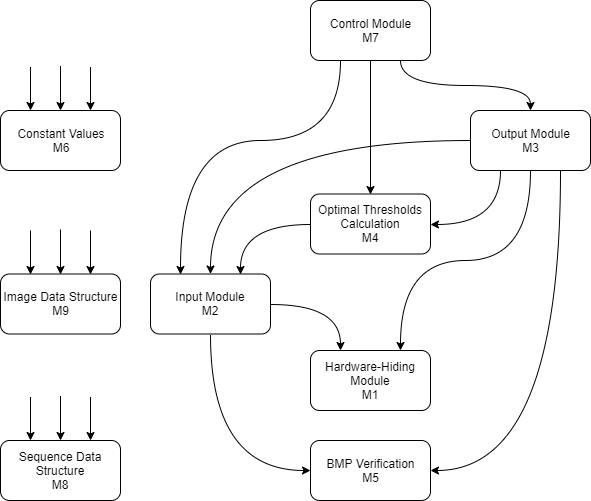
\includegraphics[width=0.7\textwidth]{UsesHierarchy.png}
\caption{Use hierarchy among modules}
\label{FigUH}
\end{figure}

%\section*{References}
\wss{MG looks good.}

\bibliographystyle {plainnat}
\bibliography{../../../refs/References}

\end{document}